\chapter[The single-underlying autocallable]{The single-underlying\\ autocallable}
\label{cap:autocallable}

The autocallable is one of the structured products most widely sold to retail investors. It is an excellent case
study because it combines digitals, a barrier put and a random maturity, and it shows sharply why the price depends on
the smile and not on the ATM volatility alone. In this chapter we decompose the product, build the closed-form oracles,
design the Black--Heston comparison with common random numbers and report the results with the Heston model calibrated
to the SPX.

\section{The term sheet}
Notional 1; all levels are ratios to a reference level $S_{\text{ref}}$ fixed at issue. Observation dates, period
lengths and fixings are
\[
0<t_1<\dots<t_n=T,\qquad\tau_i=t_i-t_{i-1},\qquad X_i=S_{t_i}/S_{\text{ref}} .
\]
Three barriers: \textbf{autocall} $B_{ac}$, \textbf{coupon} $B_c$, \textbf{protection} $B_p$. Period coupon
$c_i=c\,\tau_i$, with $c$ a simple annual rate. Every test is ``$\ge$'': being exactly on the barrier counts as above.
\begin{itemize}
\item \textbf{Intermediate dates} $t_i<T$: if $X_i\ge B_{ac}$ the product is redeemed early: it pays $1+$coupon and
terminates. Otherwise it pays the coupon if $X_i\ge B_c$.
\item \textbf{Maturity} $T$ (no autocall test): coupon if $X_n\ge B_c$; capital $1$ if $X_n\ge B_p$, otherwise $X_n$,
that is, the investor bears the full loss. The protection is \emph{European}: observed at maturity only.
\item \textbf{Memory}: an unpaid coupon is recovered on the first date on which a coupon is paid.
\end{itemize}
Every cash flow fixed at $t_i$ is paid at $t_i$ and discounted with its own $\DF(t_i)$, with no issuer credit spread.

\begin{progetto}[title={In the qpricer project: the two study term sheets}]
Both with $B_{ac}=1$, $B_c=0.7$, $B_p=0.6$, memory on, $c=8\%$ per year.
\begin{itemize}
\item \textbf{\mbox{AC-Q}}: quarterly, $t_i=i/4$, $n=6$, $T=1.5$ years, inside the last quoted expiry (1.61 years).
\item \textbf{\mbox{AC-A}}: annual, $t_i=1,2,3$. Beyond 1.61 years carry and Heston are \emph{extrapolated}: the
results must be read with this caveat.
\end{itemize}
The market inputs come from the parity table. $\ln F$ and $\ln\DF$ are interpolated linearly in $T$ and extrapolated
flat beyond the last expiry. The reference level is
\[
S_{\text{ref}}=F_0(T_{(1)})\,\DF(T_{(1)})=7374.4255
\]
(first expiry: spot minus the present value of the dividends up to there). For \mbox{AC-Q} the ratios
$f_i=F_0(t_i)/S_{\text{ref}}$ range from 1.00994 to 1.06105 and the $\DF_i$ from 0.98774 to 0.92872. The rate $c=8\%$
is used only for pricing: the fair coupon is computed separately.
\end{progetto}

\section{Cash flows on a path}
With an ``still alive'' indicator $A_i$ (starting at 1), a memory $U_i$ of unpaid coupons (starting at 0) and
$m\in\{0,1\}$ the memory flag:
\begin{align}
\chi_i&=A_i\,\ind\{X_i\ge B_{ac}\}\quad(i<n),\qquad\chi_n=0,\qquad A_{i+1}=A_i-\chi_i,\\
\pi_i&=A_i\,\ind\{X_i\ge B_c\},\qquad C_i=\pi_i\,(c_i+m\,U_i),\qquad U_{i+1}=(1-\pi_i)(c_i+m\,U_i),\\
R_i&=\chi_i\quad(i<n),\qquad R_n=A_n\big[1-(1-X_n)\,\ind\{X_n<B_p\}\big],\\
\mathrm{PV}&=\sum_i\DF_i\,(C_i+R_i),\qquad V=\E[\mathrm{PV}].\label{eq:ac-pv}
\end{align}
The order of operations matters: on each date the coupon (with memory) is computed first, then the autocall test, and
the cash flows are multiplied by $A$ \emph{before} it is updated. In this way nothing is paid twice. On an autocall date
$X_i\ge B_{ac}\ge B_c$, so an early redemption always pays the coupon as well.

\begin{esempio}[title={\texorpdfstring{Example: a path by hand (\mbox{AC-Q}, $c_i=0.02$)}{Example: a path by hand
(AC-Q, c\_i=0.02)}}]
$X_1=0.65<0.70$: no coupon, which goes into memory. $X_2=0.80$: pays $c_1+c_2=0.04$. $X_3=1.01\ge1$: redemption, pays
$1+0.02$ and terminates. If instead the path reaches maturity, a final fixing $X_6=0.65$ ($\ge0.6$ but $<0.7$) repays 1
with no coupon, while $X_6=0.40$ repays 0.40.
\end{esempio}

\paragraph{Linearity in the coupon and par coupon.} No indicator depends on $c$, which enters only through
$c_i=c\tau_i$. Hence the PV is \emph{affine} in $c$ path by path:
\begin{equation}
\mathrm{PV}_j=a_j+c\,b_j,\qquad
\hat c=\frac{1-\bar a}{\bar b},\qquad
\SE(\hat c)=\frac{s(a_j+\hat c\,b_j)}{\sqrt N\,\bar b}.
\end{equation}
The ``par'' coupon (price 1) is obtained from a single set of paths, with no root search on noisy prices; the standard
error comes from the delta method.

\section{What the investor has bought}
\subsection{The decomposition}
\noindent\textbf{Step 1 (the capital).} The redemption at maturity can be rewritten as
\[
\ind\{X\ge B_p\}+X\,\ind\{X<B_p\}=1-(1-X)\,\ind\{X<B_p\}.
\]

\noindent\textbf{Step 2 (put plus digitals).} For $B_p\le1$, on the event $\{X<B_p\}$ we have
$1-X=(B_p-X)+(1-B_p)$, hence
\[
(1-X)\,\ind\{X<B_p\}=(B_p-X)^++(1-B_p)\,\ind\{X<B_p\}:
\]
a put struck at $B_p$ plus $(1-B_p)$ \emph{digital puts} at the same strike.

\noindent\textbf{Step 3 (grouping).} Grouping the ``1'' terms by redemption date gives a bond maturing at the random
date $\tau^\star$ (autocall, or $T$):
\begin{proposizione}[Decomposition]
\begin{equation}\label{eq:ac-scomposizione}
\begin{split}
V={}&\underbrace{\E[\DF(\tau^\star)]}_{\substack{\text{bond with}\\\text{random maturity}}}
+\underbrace{\sum_i\DF_i\,\E[C_i]}_{\text{coupon digitals}}\\
&-\underbrace{\DF_n\,\E\big[A_n(1-X_n)\,\ind\{X_n<B_p\}\big]}_{\text{down-and-in put, if still alive}} .
\end{split}
\end{equation}
\end{proposizione}
Since $A_n\le1$, the embedded put is worth at most the European down-and-in put
\begin{equation}\label{eq:dip}
\mathrm{DIP}_E=\DF_n\big[p_n(B_p)+(1-B_p)\,D_n^-(B_p)\big],\qquad D_n^-(k)=\Q(X_n<k),
\end{equation}
with $p_n(k)=\E(k-X_n)^+$. This piece is \textbf{static and model-free}: given the smile at maturity $T$, it is a put
plus $0.4$ digital puts at 60\%.

\begin{idea}[title={Who is long what}]
The \textbf{investor} is long the bond and the coupon digitals, and \textbf{short} a 60\% down-and-in put: they have
sold the issuer protection against crashes, and this is what funds high coupons. They are short volatility and short
the downside. The \textbf{issuer} holds the opposite position: long the put, short the digitals and the bond. At issue
it is long vega. When the market falls its vega grows, reaches a maximum above the barrier and then changes sign,
because close to maturity the put becomes an in-the-money digital (``peak vega''). Issuers hedge by selling
volatility: autocallable issuance is a steady supply of volatility to the market.
\end{idea}

\subsection{The sign of vega: clear without autocall, not with it}
With $s$ the total volatility, let
\[
d_\pm(f,L,s)=\frac{\ln(f/L)\pm s^2/2}{s},\qquad
\partial_sd_-=-\frac{\ln(f/L)}{s^2}-\frac12 .
\]
The derivative is negative exactly when $L<f\,e^{s^2/2}$. In that case the ``above'' digital $\Phi(d_-)$ loses value
with volatility and the ``below'' digital $\Phi(-d_-)$ gains value. With positive carry ($f_i\ge1$) this holds for the
coupon digitals at $B_c$, for the autocall digitals at $B_{ac}=1$ and for the put at $B_p$. Hence, \textbf{without
autocall}, $V$ is strictly decreasing in $\sigma$: the investor is short vega. With the autocall there is no general
sign, because volatility also shifts the timing of the redemption (see Section~\ref{sec:ac-vega}).

\section{Why a flat volatility is not enough}
The digital is the derivative of the put with respect to the strike. If the put price is $p_{BS}(k,\sigma(k))$, with a
strike-dependent volatility, the chain rule gives
\begin{equation}\label{eq:digitale-smile}
D^-(k)=\frac{\partial p}{\partial k}
=\underbrace{\Phi(-d_-)}_{\text{Black at level }\sigma(k)}
+\underbrace{k\,\varphi(d_-)\sqrt t\,\sigma'(k)}_{\text{smile slope}} .
\end{equation}
The first term is $\partial_kp_{BS}$, the second is the vega of the put, $k\varphi(d_-)\sqrt t$, times $\sigma'(k)$.
\begin{perche}[title={Why no single volatility prices a digital}]
The price of a digital depends not only on the \emph{level} of the volatility at the strike, but also on the
\emph{slope} of the smile there. With the SPX skew ($\sigma'<0$) the second term matters. Using a single volatility
for everything, the ATM one to boot, is therefore wrong twice over: the 60\% put and the 70\% coupon sit deep in the
skew, where the implied volatility is much higher than ATM.
\end{perche}
The expected sign is therefore $V_{\text{Heston}}<V_{\text{Black}}(\sigma_{\mathrm{ATM}})$. The fatter left tail makes
the put sold by the investor worth more and lowers the probability of being above $B_c$. Near ATM, on the other hand,
with $\sigma'<0$ \eqref{eq:digitale-smile} says that the autocall digital $D^+(1)$ is above its flat value: more early
redemptions.

\section{The closed-form oracles}
Before trusting the Monte Carlo on the full product, one checks cases that can be computed exactly.
\begin{itemize}
\item \textbf{No autocall and no memory} ($B_{ac}=\infty$, $m=0$). Each cash flow depends on a single fixing, so the
value is a sum of marginals:
\begin{equation}\label{eq:ac-nocall}
V^{nc}=\sum_i\DF_i\,c_i\,D_i^+(B_c)+\DF_n-\mathrm{DIP}_E .
\end{equation}
Under Black
\[
D_i^+(k)=\Phi\big(d_-(f_i,k,s_i)\big),\qquad\mathrm{DIP}_E=\DF_n\big[\Phi(-d_-)-f_n\Phi(-d_+)\big],
\]
with $d_\pm=d_\pm(f_n,B_p,s_n)$. Under Heston puts and digitals come from COS (Chapter~\ref{cap:heston}); the digital
is a central difference from \emph{a single} COS call at the three strikes, so it is the derivative of one series.
\item \textbf{Two dates}, any memory. One conditions on $X_1$: given $X_1=x$, the fixing $X_2$ is lognormal with mean
$g=xf_2/f_1$ and total volatility $s_{1,2}$, so the cash flows at $t_2$ are priced with Black. What remains is a
one-dimensional integral over the law of $X_1$, split at the jump point of the memory ($X_1=B_c$).
\item \textbf{Zero volatility}: $X_i=f_i$ and the term sheet is evaluated by hand.
\item \textbf{Path identities}: the sum of the first-redemption probabilities plus the probability of reaching
maturity equals 1 exactly; the PV is monotonic in $B_c$, $B_p$, $c$ and in the memory.
\end{itemize}

\section{Monte Carlo and common random numbers}
Under Black one exact step per period is enough. Under Heston one uses QE-M with sub-steps $\Delta\le1/32$ that end
exactly on the observation dates.

\subsection{The common-random-numbers design}
We want the \emph{difference} $V_H-V_{BS}$, which is of the order of 1--2\% of the notional. With independent seeds
its variance would be the sum of the two variances. With common random numbers (CRN) it is estimated on the per-path
differences.

\noindent\textbf{Step 1.} At each sub-step $k$ of length $\Delta_k$, QE-M draws independent $(Z_{v,k},Z_{\perp,k})$;
the spot shock is $\rho Z_{v,k}+\sqrt{1-\rho^2}Z_{\perp,k}$, which is $\N(0,1)$.

\noindent\textbf{Step 2.} For period $i$ the Brownian increments are summed and normalized:
\begin{equation}\label{eq:crn}
Z_i=\sum_{k\in\text{period }i}\sqrt{\frac{\Delta_k}{\tau_i}}\,\big(\rho Z_{v,k}+\sqrt{1-\rho^2}\,Z_{\perp,k}\big).
\end{equation}
A sum of independent $\N(0,\Delta_k)$ is $\N(0,\tau_i)$, so $Z_i$ is exactly $\N(0,1)$, and independent across
different periods.

\noindent\textbf{Step 3.} The Black paths are built with these $Z_i$: they are exact GBMs, driven by the Brownian
motion of the Heston spot. The difference $D_j=\mathrm{PV}^H_j-\mathrm{PV}^{BS}_j$ has standard error $s_D/\sqrt N$,
\emph{never} $\sqrt{\SE_H^2+\SE_{BS}^2}$, which holds only for independent estimates.

\begin{attenzione}[title={The gain is modest, and that is fine}]
The digitals limit the correlation: paths close to a barrier change outcome between the two models. On the full
product (calibrated \mbox{AC-Q}) the error of the difference is 0.000217, just below what the separate SEs would give
(0.000229 for Heston, 0.000094 for Black). On the term in which both legs are lognormal the gain is instead large: SE
0.000120 against separate SEs of 0.000163 and 0.000094. The real benefit is consistency: every term of the
decomposition that follows is a per-path difference, so it measures model differences and not noise.
\end{attenzione}

\section{Black versus Heston: the attribution}
Three prices are compared on the same paths:
\begin{itemize}
\item $V_{BS}$: Black with flat volatility $\sigma_{\mathrm{ATM}}$, the Heston implied volatility at the forward and at
maturity $T$. In this way both models price the ATM-forward vanilla at $T$ identically.
\item $V_{TS}$: Black with the Heston expected variance \eqref{eq:var-attesa},
\[
w(t)=\theta t+(v_0-\theta)\,\frac{1-e^{-\kappa t}}{\kappa},
\]
that is, the limit $\xi\to0$.
\item $V_H$: Heston.
\end{itemize}
The superscript ``nc'' denotes the same term sheet without autocall and without memory, priced in closed form with
\eqref{eq:ac-nocall}. The difference decomposes exactly into three terms:
\begin{equation}\label{eq:attribuzione}
\begin{split}
V_H-V_{BS}={}&\underbrace{(V_{TS}-V_{BS})}_{\substack{\text{1: flat }\sigma_{\mathrm{ATM}}\text{ vs}\\\text{variance curve}}}
+\underbrace{(V^{nc}_H-V^{nc}_{TS})}_{\substack{\text{2: marginal smile}\\\text{at }B_p,\,B_c}}\\
&+\underbrace{\big[(V_H-V_{TS})-(V^{nc}_H-V^{nc}_{TS})\big]}_{\text{3: path (forward skew, vol-of-vol)}} .
\end{split}
\end{equation}
\begin{itemize}
\item \textbf{Term 1} compares the flat volatility with the Heston expected-variance curve. It contains a \emph{level}
part ($\sqrt{w(T)/T}$ against $\sigma_{\mathrm{ATM}}$: the Heston ATM implied volatility is below the square root of
the expected variance because of the vol-of-vol) and a \emph{shape} part.
\item \textbf{Term 2} is the difference of two closed forms, so it has no standard error. It measures the smile at the
barriers: the Heston put and digitals against those of a lognormal with the same variance.
\item \textbf{Term 3} is the residual. Every coupon and the put pay only on paths not yet redeemed, that is, paths
that stayed below 100\%. The price therefore depends on the future \emph{conditional} distribution (the forward skew),
which Heston generates and Black does not.
\end{itemize}
Since term 3 is defined as a residual, the sum adds back to the difference by construction: this is not a test. The
real tests are the legs compared with the closed forms.

\subsection{The results with calibrated Heston}
The parameters come from the calibration of Chapter~\ref{cap:calibrazione} (SPX snapshot, 21 expiries with
$T\ge0.1$): $\kappa=4.575$, $\theta=0.05293$, $\xi=1.648$, $\rho=-0.7518$, $v_0=0.05237$. Table~\ref{tab:ac-risultati} reports the results with $2\times10^5$ paths.
\begin{table}[htbp]
\centering
\small
\caption{Black versus calibrated Heston on the two study term sheets ($2\times10^5$ paths; CRN standard errors in
brackets).}
\label{tab:ac-risultati}
\begin{tabularx}{\textwidth}{>{\raggedright\arraybackslash}Xll}
\toprule
& \mbox{AC-Q} (1.5 years) & \mbox{AC-A} (3 years, extrapolated)\\
\midrule
$\sigma_{\mathrm{ATM}}$ (Heston) / $\sqrt{w(T)/T}$ & 18.85\% / 22.99\% & 19.72\% / 23.00\%\\
$V_{BS}$ & 1.014530 & 1.021479\\
$V_{TS}$ & 1.006324 & 1.002757\\
$V_H$ & 0.995842 & 0.996342\\
difference $V_H-V_{BS}$ (CRN SE) & $-0.018688$ (0.000217) & $-0.025137$ (0.000342)\\
1: flat $\sigma_{\mathrm{ATM}}$ vs variance curve & $-0.008206$ (0.000120) & $-0.018722$ (0.000163)\\
2: marginal smile (exact) & $-0.020445$ & $-0.014800$\\
3: path & $+0.009963$ (0.000216) & $+0.008386$ (0.000364)\\
par coupon Black / Heston & 5.60\% / 8.93\% & 6.58\% / 8.29\%\\
coupon difference (SE) & $+3.33\%$ (0.05\%) & $+1.71\%$ (0.03\%)\\
$P$(redemption at $t_1$) Black / Heston & 0.5222 / 0.6814 & 0.5395 / 0.6755\\
$P$(never redeemed) Black / Heston & 0.2164 / 0.1371 & 0.3273 / 0.2247\\
expected life Black / Heston & 0.643 / 0.503 years & 1.788 / 1.549 years\\
\bottomrule
\end{tabularx}
\end{table}


\begin{figure}[htbp]
\centering
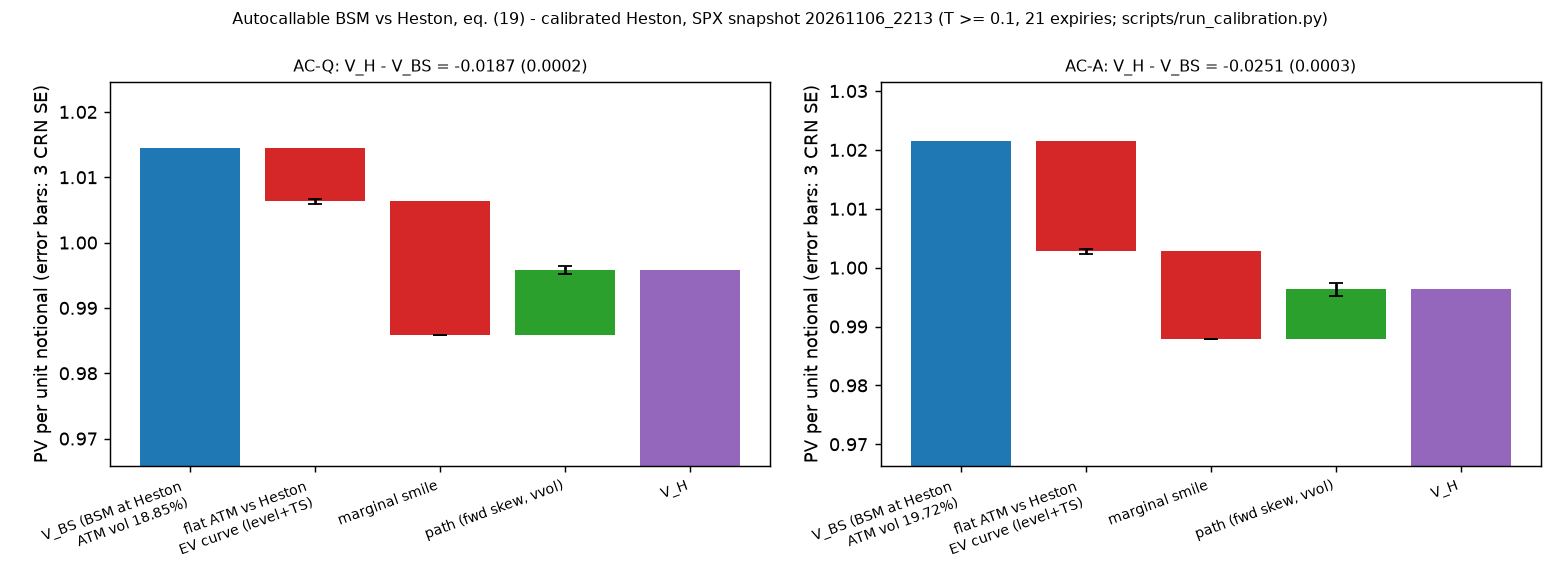
\includegraphics[width=\textwidth]{autocall_attribution_heston_fit_20261106_2213.png}
\caption{Attribution \eqref{eq:attribuzione} with Heston calibrated to the SPX, for \mbox{AC-Q} (left) and
\mbox{AC-A} (right). From the left: $V_{BS}$ at the Heston ATM volatility, the three terms (error bars at 3 CRN SE)
and $V_H$.}
\label{fig:ac-attribuzione}
\end{figure}

\paragraph{How to read them.} Figure~\ref{fig:ac-attribuzione} shows the waterfall. On \mbox{AC-Q} Heston is worth
1.87\% of notional less than Black, in the expected direction.
\begin{itemize}
\item \textbf{Term 2} dominates ($-0.0204$): it is the skew at the 60\% and 70\% barriers. The left tail makes the
issuer's put more expensive and the coupons less likely.
\item \textbf{Term 1} ($-0.0082$) is almost all level: $v_0\approx\theta$, so the curve $w(t)/t$ is almost flat, and
the difference between 22.99\% and 18.85\% is the vol-of-vol effect, very large in the fit ($\xi=1.65$).
\item \textbf{Term 3} is positive ($+0.0100$) and offsets about a third of the rest. It also contains the fact that the
product without autocall suffers the smile penalty on all paths, while the product with autocall suffers it only on
the surviving ones.
\item Heston redeems much more often on the first date (68\% against 52\%): with $\sigma'<0$ the ATM digital is above
its flat value. The expected life shortens.
\item The \textbf{par coupon} rises from 5.60\% to 8.93\%: a flat ATM volatility would make the issuer offer a coupon
more than 3 points too low.
\end{itemize}

\paragraph{Which volatility for Black?} The choice of $\sigma_{\mathrm{ATM}}$ matters, and this is why sensitivity rows
are reported (\mbox{AC-Q}, Table~\ref{tab:ac-sens}).
\begin{table}[htbp]
\centering
\small
\caption{Sensitivity of $V_{BS}$ (\mbox{AC-Q}) to the volatility chosen for Black.}
\label{tab:ac-sens}
\begin{tabularx}{\textwidth}{Xrr}
\toprule
Black volatility & $\sigma$ & $V_{BS}$\\
\midrule
Heston ATM at the forward (the reference leg) & 18.85\% & 1.014530\\
market ATM interpolated at 1.5 years & 18.29\% & 1.015253\\
Heston at the strike $S_{\text{ref}}$ & 20.37\% & 1.012036\\
Heston at the barrier $B_pS_{\text{ref}}$ & 31.79\% & 0.977950\\
\bottomrule
\end{tabularx}
\end{table}

The Heston fit sits about 0.65 vol points above the market ATM on the last expiry (18.94\% against 18.29\%). At the
market ATM volatility $V_{BS}$ rises by 0.000723 (about 3.3 CRN SE of the difference) and the difference with Heston
becomes $-0.019411$: the conclusion does not change. Black at the barrier volatility instead overshoots
($0.977950<V_H$): that volatility prices the put, but the coupons and redemptions sit at other strikes, and the digital
also needs the slope. On \mbox{AC-A} the market ATM volatility is not available (no quoted expiry beyond 1.61 years);
the other two rows give 1.011832 (21.47\%) and 0.967614 (28.36\%).

\begin{progetto}[title={In the qpricer project: checks on the calibrated comparison}]
\begin{itemize}
\item Black and deterministic-variance legs on the CRN paths, restricted to the first two dates, against the two-date
formula: $\max|z|=0.20$ (\mbox{AC-Q}) and 0.72 (\mbox{AC-A}). No-autocall legs on the paths against
\eqref{eq:ac-nocall}: $\max|z|=0.87$ and 1.19.
\item An independent check recomputed everything with its own methods: exact value of $V_{BS}$ by backward induction
1.014493 (project Monte Carlo at $z=0.40$); $V_H=0.995882$ with its own QE-M scheme (project at $z=-0.16$); difference
$-0.018611$; term 2 within $4\times10^{-10}$. With step $1/256$ $V_H=0.995905$: no step bias.
\item Effect of a small known inconsistency: $S_{\text{ref}}$ uses the discount factor of the first expiry from
parity, which is slightly biased; with the smoothed curve $S_{\text{ref}}$ would rise by 0.074\%. The measured effect
on the \mbox{AC-Q} difference is $-8\times10^{-5}$, that is 0.4 CRN SE.
\end{itemize}
\end{progetto}

\section{No single sign for vega}
\label{sec:ac-vega}
Without autocall the product is strictly decreasing in $\sigma$ (tested in closed form). On the full product it is not.
A grid of $\sigma$ under Black, with common random numbers across grid points, gives the values of Table~\ref{tab:ac-vega}.
\begin{table}[htbp]
\centering
\small
\caption{Value of the two autocallables under Black as the flat volatility $\sigma$ varies.}
\label{tab:ac-vega}
\begin{tabular*}{\textwidth}{@{\extracolsep{\fill}}lccccccc@{}}
\toprule
$\sigma$ & 0.10 & 0.15 & 0.20 & 0.25 & 0.30 & 0.35 & 0.40\\
\midrule
$V$ (\mbox{AC-Q}) & 1.01730 & 1.01773 & 1.01271 & 1.00072 & 0.98433 & 0.96618 & 0.94767\\
$V$ (\mbox{AC-A}) & 1.04433 & 1.04008 & 1.01997 & 0.98996 & 0.95633 & 0.92251 & 0.88936\\
\bottomrule
\end{tabular*}
\end{table}

It is a pure Black computation on the market inputs, in which no Heston parameter plays any role. On \mbox{AC-Q} the
value \emph{rises} from $\sigma=0.10$ to $0.15$ ($+0.00043$, SE of the difference 0.00004) and then falls. On
\mbox{AC-A} it is monotonic.
\begin{perche}[title={Why vega changes sign}]
It is a timing effect. For $\sigma\to0$ the \mbox{AC-Q} product is redeemed with certainty on the first date, because
$f_1=1.00994\ge1$. A little volatility delays the redemption, and the investor collects for longer an 8\% coupon,
higher than the fair one, before the put starts to weigh. Only with more volatility does the sold put prevail. Hence
``the autocallable is short vega'' is true for the investor on the product without autocall, not in general.
\end{perche}

\section{A published value that does not reproduce}
Deng, Mallett and McCann (2011), ``Case 2'': monthly dates for one year, $B_{ac}=B_c=1.02$, memory, accrual coupons
$c_j=e^{0.092t_j}-e^{0.092t_{j-1}}$, European protection $B_p=0.8$, $\sigma=20\%$, $F_0(t)=100e^{0.04t}$,
$\DF(t)=e^{-0.06t}$ (the discount factor includes the issuer's CDS spread).
\begin{itemize}
\item Project Monte Carlo: 97.508 (SE 0.009, $10^6$ paths).
\item Exact value, computed independently by backward induction: 97.507 (between the two, $z=+0.09$).
\item Published value (explicit finite differences): \textbf{98.39}, about 100 SE away.
\end{itemize}
The rest of the paper, on the other hand, does reproduce: ``Case 1'' (without autocall) gives roughly par (99.976),
and the first-redemption probabilities of their table 1 match ($\max|z|=2.11$; the first one, $p_1=0.3767$, can also
be derived by hand). Two independent implementations agree with each other and not with the published value. The
possible causes are a different coupon or protection convention in the paper, or the finite-difference error, whose
accuracy the paper does not state. Nothing was adjusted to make it match; the value is not used as an oracle.

\section{Model risk}
\begin{itemize}
\item \textbf{What the vanillas pin down.} Today's vanilla prices pin down the marginals: the European down-and-in put
is a put plus digitals from the smile at $T$ \eqref{eq:dip}, and this is term 2. They do not pin down term 3: coupons
and put pay only on paths that stayed below 100\%, so the price depends on the \emph{forward} skew, driven by
vol-of-vol and spot--vol correlation.
\item \textbf{Heston cannot move it on its own.} In Heston $\xi$ and $\rho\xi$ are fixed by the vanilla fit. Two models
calibrated to the same prices (local volatility, whose forward skew is flat, and stochastic volatility) can give
different prices: this is model risk, which a local-stochastic volatility model would make it possible to control.
\item \textbf{Extrapolation.} \mbox{AC-A} goes beyond the last quoted expiry: carry and Heston are extrapolated.
\item \textbf{Credit and Greeks.} No issuer spread in the discounting. The Greeks are unstable, because the payoff is
made of digitals: pathwise derivatives lose the Dirac terms, and finite differences have a variance that grows like
$1/h$. Dedicated methods are needed (likelihood ratio, digital smoothing), outside the scope of the project.
\end{itemize}

\begin{progetto}[title={In the qpricer project: code and checks}]
The code:

\noindent{\small\begin{tabularx}{\linewidth}{@{}l>{\raggedright\arraybackslash}X@{}}
\path{src/qpricer/products.py} & cash flows (\code{autocall\_flows})\\
\path{src/qpricer/engines/exotic_mc.py} & Monte Carlo and CRN (\code{autocall\_mc}, \code{fixings})\\
\path{src/qpricer/engines/analytic.py} & oracles (\code{autocall\_nocall}, \code{autocall\_two\_dates})\\
\path{scripts/autocall_compare.py} & Black--Heston comparison\\
\path{tests/test_autocallable.py} & tests
\end{tabularx}}
\medskip

\noindent The checks:
\begin{itemize}
\item Black Monte Carlo against the closed forms (no autocall, $n=1$, two dates with and without memory):
$\max|z|=1.79$.
\item Heston: mean of $M_t$ equal to 1, digitals against COS, product without autocall against COS: $\max|z|=1.32$.
\item Heston with $\xi=10^{-4}$ against Black at the discrete QE variance, same draws: $|z|=0.18$.
\item Cash flows identical (within $10^{-15}$) to an independent path-by-path transcription, on $20{,}000$ paths and
seven term-sheet variants, with exact ties at every barrier.
\item Full product under Black against an independent exact value, 18 cases: $\max|z|=2.36$.
\end{itemize}
\end{progetto}

\needspace{6\baselineskip}
\begin{riassunto}
\begin{itemize}
\item Autocallable = random-maturity bond + coupon digitals $-$ 60\% European down-and-in put.
\item The investor is short the put and short the downside; the issuer is long vega at issue (``peak vega'' above the
barrier). Without autocall the investor is short vega; with the autocall there is no single sign.
\item Digitals depend on the smile slope: no single volatility prices them.
\item PV affine in the coupon $\Rightarrow$ par coupon from a single set of paths.
\item CRN: Black driven by the Heston spot shocks; SE always from the per-path differences.
\item With calibrated Heston (\mbox{AC-Q}): $V_H-V_{BS}=-0.0187$, of which smile at the barriers $-0.0204$; fair coupon
from 5.60\% to 8.93\%. The path term is model risk.
\end{itemize}
\end{riassunto}

\needspace{6\baselineskip}
\begin{domande}[before skip=6pt plus 8pt]
\begin{enumerate}
\item Decompose an autocallable into simple instruments. Who is long vega?
\item Derive the decomposition of the capital into a put plus digitals.
\item Why is the ATM volatility not the relevant one? What does the smile slope add to a digital?
\item Why is the par coupon obtained without a root search?
\item Show that the $Z_i$ of \eqref{eq:crn} are independent $\N(0,1)$. Why is the SE of the difference not
$\sqrt{\SE_H^2+\SE_{BS}^2}$?
\item What does each term of \eqref{eq:attribuzione} measure? Which one is not pinned down by today's vanillas?
\item Why is the \mbox{AC-Q} product worth more at $\sigma=0.15$ than at $\sigma=0.10$?
\item A published value is 100 SE away from yours and from an independent computation: what do you do?
\end{enumerate}
\end{domande}
